% Springer/Quarto PDF header includes.
%
% Quarto owns execution, assembly, cross-references, and bibliography wiring.
% Springer remains the PDF class contract through documentclass: SNmono in
% _quarto.yml. Keep publisher-specific LaTeX here rather than in chapters.

\usepackage{type1cm}
\usepackage{array}
\usepackage{float}
\usepackage{placeins}
\usepackage{needspace}
\usepackage[bottom]{footmisc}
% Resolve the SNmono vs sidenotes clash: Springer's class predefines
% \sidecaption, which the sidenotes package (loaded by Quarto's
% reference-location: margin) then tries to redefine. Free the name first.
\let\sidecaption\undefined
% === arch2 layout auto-fix: automatic margin-note overflow control ===
% With reference-location: margin, Quarto places footnotes as marginals. A
% sidenote carrying no manual offset (the normal case) is routed through
% \marginpar by the sidenotes package, so marginfix can manage it. marginfix
% tracks the free vertical space in each margin and automatically shifts notes
% (an automatic vertical offset) so they never run off the page bottom or
% collide. This is the render-time counterpart to the layout audit's
% footnote-overflow / physical-bleed checks, which detect the same failures.
\usepackage{marginfix}
% Route .column-margin asides (Quarto emits raw \marginnote) through the same
% marginfix-managed \marginpar as the footnotes. This makes the asides (a) auto-
% offset so they never run off the page or collide with footnotes, and (b) follow
% the outer-margin alternation instead of always sitting on the right, which put
% them on the inner margin of verso pages. Done \AtBeginDocument so it runs after
% Quarto has loaded marginnote/sidenotes.
\AtBeginDocument{\RenewDocumentCommand{\marginnote}{o +m o}{\marginpar{#2}}}
\usepackage{xcolor}
% Footnote margin-mark styling: a small bottom-left corner bracket (an "L")
% around just the sidenote number, which sits in its nook; the note text then
% flows normally. A short left rule and a short bottom rule, both ~number height,
% meet at the corner in the book's accent blue for a touch of personality.
% Targets sidenote footnotes (\@sidenotes@placemarginal); .column-margin asides
% route through the \marginnote redefinition and stay unbracketed.
\newcommand{\archsnframe}[1]{%
  {\color{archtwoblue}\rule[-0.15ex]{0.4pt}{1.35ex}\rule[-0.15ex]{5pt}{0.4pt}}%
  \hspace{2pt}#1%
}
\makeatletter
\AtBeginDocument{\RenewDocumentCommand{\@sidenotes@placemarginal}{+m +m}{\marginpar{\archsnframe{#2}}}}
\makeatother
\usepackage{fontawesome5}
\usepackage[most]{tcolorbox}
\usepackage{tikz}
\usetikzlibrary{arrows.meta,calc,positioning,shapes.geometric}
\usepackage{newtxtext}
\usepackage[varvw]{newtxmath}
\renewcommand{\ttdefault}{cmtt}

\bibpunct{(}{)}{;}{a}{,}{,}
\AtBeginDocument{%
  \makeatletter
  \def\bibsection{\subsection*{\refname}\markright{\refname}%
    \csname biblst@rthook\endcsname\par}%
  \makeatother
}
\SuppressSpringerImprint
% Preview version: the publish pipeline injects \ArchTwoReleaseVersion (from
% ARCH2_VERSION, via cli/arch2.py header-includes) so the PDF matches the site;
% local builds fall back to the static default below. \SetArchTwoPreviewVersion
% stores the token unresolved, so it resolves at footer/title time regardless of
% where the injected \def lands in the preamble.
\providecommand{\ArchTwoReleaseVersion}{Preview v0.1.0}
\SetArchTwoPreviewVersion{\ArchTwoReleaseVersion}
\newcommand{\ArchTwoSiteURL}{arch2.mlsysbook.ai}

\definecolor{archtwoink}{HTML}{20252B}
\definecolor{archtwomuted}{HTML}{59636D}
\definecolor{archtwoblue}{HTML}{1F5F7A}
\definecolor{archtwobluefill}{HTML}{EEF7FB}
\definecolor{archtwogreen}{HTML}{4B7F52}
\definecolor{archtwogreenfill}{HTML}{F1F8F0}
\definecolor{archtwoorange}{HTML}{A9671E}
\definecolor{archtwoorangefill}{HTML}{FFF6E8}
\definecolor{archtwoline}{HTML}{9AA8B5}
\definecolor{archtwopanel}{HTML}{F7FAFB}
\definecolor{archtwogrid}{HTML}{E2E8ED}
\definecolor{archtwoevidence}{HTML}{7E6AA8}
\definecolor{archtwoevidencefill}{HTML}{F4F1FA}
\definecolor{archtwoodanger}{HTML}{C44E52}
\definecolor{archtwoodangerfill}{HTML}{F8EAEA}

% Hyperlinks: keep cross-references, citations, and URLs clickable, but render
% them in black rather than the default blue. Deferred with \AtBeginDocument so it
% overrides Quarto's own hyperref setup regardless of load order.
\AtBeginDocument{\hypersetup{colorlinks=true,allcolors=black}}

% Widen the TOC section/subsection number columns. The class sizes \tocsecnum for
% "88.8" (two-digit chapter, one-digit section), so two-digit sections like 10.13
% collide with the title. Bump the number widths and recompute the indents via the
% class's own \calctocindent so the dotted leaders stay aligned.
\makeatletter
\tocsecnum=30\p@
\tocsubsecnum=37\p@
\calctocindent
\makeatother

% Wrap long code-listing lines so they never bleed past the right margin. Quarto
% highlights code with base fancyvrb, whose Verbatim has no line breaking; load
% fvextra (a drop-in extension) to get breaklines/breakanywhere.
\usepackage{fvextra}
\fvset{breaklines=true,breakanywhere=true}

\newcommand{\ArchTwoRule}{%
  \vskip 3.2pt%
  \hbox to\textwidth{%
    {\color{archtwoblue}\rule{0.72in}{0.7pt}}%
    {\color{archtwoline}\rule{\dimexpr\textwidth-0.72in\relax}{0.35pt}}%
  }%
}

\newcommand{\ArchTwoRunningFooter}{%
  \vbox{%
    {\color{archtwoline}\hrule height 0.25pt}%
    \vskip 3.4pt%
    \hbox to\textwidth{%
      \normalfont\sffamily\tiny\color{archtwomuted}Architecture 2.0 | \ArchTwoPreviewVersion%
      \hfil
      \ArchTwoSiteURL%
    }%
  }%
}

\newcommand{\ArchTwoChapterFooter}{%
  \vbox{%
    {\color{archtwoline}\hrule height 0.25pt}%
    \vskip 3.4pt%
    \hbox to\textwidth{%
      \normalfont\sffamily\tiny\color{archtwomuted}Architecture 2.0 | \ArchTwoPreviewVersion%
      \hfil
      {\color{archtwoblue}\bfseries\thepage}%
    }%
  }%
}

\newcommand{\ArchTwoCoverMotif}{%
  \begingroup
  \sffamily
  \begin{tikzpicture}[
    x=1cm,
    y=1cm,
    >=Stealth,
    arrow/.style={-{Stealth[length=4.5pt,width=5.5pt]}, line width=0.8pt, draw=archtwoblue},
    feedback/.style={-{Stealth[length=4.5pt,width=5.5pt]}, line width=1.1pt, draw=archtwoblue},
    motiflabel/.style={fill=archtwopanel, fill opacity=0.92, text opacity=1, inner xsep=2pt, inner ysep=1pt}
  ]
    \fill[archtwopanel] (0,0) rectangle (10.85,4.48);
    \draw[archtwoline, line width=0.6pt] (0,0) rectangle (10.85,4.48);
    \foreach \x in {1.05,2.10,3.15,4.20,5.25,6.30,7.35,8.40,9.45} {
      \draw[archtwogrid, line width=0.25pt] (\x,0.46) -- (\x,3.82);
    }
    \foreach \y in {1.15,1.90,2.65,3.40} {
      \draw[archtwogrid, line width=0.25pt] (0.42,\y) -- (10.43,\y);
    }

    \node[anchor=north west, font=\tiny\bfseries, text=archtwomuted] at (0.42,4.22)
      {HUMAN-GOVERNED ARCHITECTURE LOOP};

    \coordinate (center) at (5.425, 2.24);

    \fill[archtwobluefill, opacity=0.55] (3.00,0.56) rectangle (5.425,3.76);
    \fill[archtwogreenfill, opacity=0.55] (5.425,0.56) rectangle (7.85,3.76);
    \node[anchor=north east, font=\tiny\bfseries, text=archtwomuted] at (10.43,4.22) {AGENT + TOOLS};

    \draw[archtwoline, line width=0.6pt, dash pattern=on 3pt off 2pt] (center) circle (1.3cm);

    \coordinate (intent) at (4.506, 3.159);
    \coordinate (synthesis) at (6.344, 3.159);
    \coordinate (evidence) at (6.344, 1.321);
    \coordinate (decide) at (4.506, 1.321);

    \node[circle, draw=archtwoink, fill=white, line width=1.0pt, minimum size=0.9cm] (N-intent) at (intent) {};
    \node[circle, draw=archtwoblue, fill=white, line width=0.9pt, minimum size=0.9cm] (N-synthesis) at (synthesis) {};
    \node[circle, draw=archtwoblue, fill=white, line width=0.9pt, minimum size=0.9cm] (N-evidence) at (evidence) {};
    \node[circle, draw=archtwoink, fill=white, line width=1.0pt, minimum size=0.9cm] (N-decide) at (decide) {};

    % Font Awesome icons read more reliably than tiny hand-drawn glyphs at cover scale.
    \node[font=\Large, text=archtwoink, inner sep=0pt] at (2.58,2.22) {\faUserTie};
    \node[font=\Large, text=archtwoblue, inner sep=0pt] at (8.40,2.24) {\faRobot};

    \node[font=\normalsize, text=archtwoink, inner sep=0pt] at (intent) {\faIcon{bullseye}};
    \node[font=\normalsize, text=archtwoblue, inner sep=0pt] at (synthesis) {\faIcon{robot}};
    \node[font=\normalsize, text=archtwoblue, inner sep=0pt] at (evidence) {\faIcon{check}};
    \node[font=\normalsize, text=archtwoink, inner sep=0pt] at (decide) {\faIcon{code-branch}};

    \draw[arrow] (N-intent) to[bend left=22] (N-synthesis);
    \draw[arrow] (N-synthesis) to[bend left=22] (N-evidence);
    \draw[arrow] (N-evidence) to[bend left=22] (N-decide);
    \draw[feedback] (N-decide) to[bend left=22] (N-intent);

    \node[motiflabel, left=0.22cm of N-intent, font=\scriptsize\bfseries, text=archtwoink, align=right] (L-intent) {
      Architect's Intent \\[-3pt] \tiny\color{archtwomuted}\textnormal{Human Goal}
    };

    \node[motiflabel, right=0.22cm of N-synthesis, font=\scriptsize\bfseries, text=archtwoink, align=left] (L-synthesis) {
      Agent Synthesis \\[-3pt] \tiny\color{archtwomuted}\textnormal{Exploration \& Tools}
    };

    \node[motiflabel, right=0.22cm of N-evidence, font=\scriptsize\bfseries, text=archtwoink, align=left] (L-evidence) {
      System Evidence \\[-3pt] \tiny\color{archtwomuted}\textnormal{Fidelity \& Metrics}
    };

    \node[motiflabel, left=0.22cm of N-decide, font=\scriptsize\bfseries, text=archtwoink, align=right] (L-decide) {
      Loop Decision \\[-3pt] \tiny\color{archtwomuted}\textnormal{Accept / Reject / Escalate}
    };

  \end{tikzpicture}%
  \endgroup
}

\makeatletter
\def\@maketitle{%
  \thispagestyle{empty}%
  \begingroup
    \parindent=\z@
    \color{archtwoink}%
    \begin{tikzpicture}[remember picture,overlay]
      \fill[archtwoblue] ([xshift=0.76in,yshift=-0.58in]current page.north west)
        rectangle ([xshift=0.82in,yshift=1.12in]current page.south west);
    \end{tikzpicture}%
    \vspace*{-0.56in}%
    {\large\@author\par}%
    \vspace{0.10in}%
    {\small\bfseries\color{archtwoblue}PREVIEW EDITION\par}%
    \vspace{0.62in}%
    {\color{archtwoblue}\rule{0.78in}{1.2pt}\par}%
    \vspace{0.18in}%
    {\fontsize{35}{39}\selectfont\bfseries\@title\par}%
    \vspace{0.28in}%
    \if!\@subtitle!\else
      {\Large\color{archtwomuted}\@subtitle\par}%
      \vspace{0.62in}%
    \fi
    \ArchTwoCoverMotif\par
    \vfill
    {\color{archtwoline}\rule{\textwidth}{0.45pt}\par}%
    \vspace{0.14in}%
    {\small\bfseries Work in progress\par}%
    \vspace{0.10in}%
    {\small\color{archtwomuted}\ArchTwoPreviewVersion\ for the ISCA 2026 Architecture 2.0 workshop.\par}%
    \ifx\@date\@empty\else
      \vspace{0.10in}%
      {\small\color{archtwomuted}\@date\par}%
    \fi
    \vspace*{0.40in}%
  \endgroup
}

\def\@makechapterhead#1{{\parindent\z@\raggedright\normalfont
  \hyphenpenalty \@M
  \interlinepenalty\@M
  \if@chapnum
     \chapnumsize\chapnumstyle
     \@chapapp\ \thechapter\thechapterend\par
     \vskip 2\p@
  \fi
  \chapsize\chapstyle
  \ignorespaces#1\par\nobreak
  \vskip 8\p@
  {\color{archtwoblue}\rule{0.72in}{1.0pt}\par}%
  \processchapsubtit
  \processchapauthor
  \processmotto
  \vskip 18\p@}}

\def\@makeschapterhead#1{{\parindent \z@ \raggedright\normalfont
  \hyphenpenalty \@M
  \interlinepenalty\@M
  \chapsize\chapstyle
  \ignorespaces#1\par\nobreak
  \vskip 8\p@
  {\color{archtwoblue}\rule{0.72in}{1.0pt}\par}%
  \processmotto
  \vskip 18\p@}}

\def\ps@bchap{%
  \let\@oddhead\@empty\let\@evenhead\@empty
  \def\@oddfoot{\ArchTwoChapterFooter}%
  \let\@evenfoot\@oddfoot}

\def\ps@headings{\let\@mkboth\markboth
   \def\@oddfoot{\ArchTwoRunningFooter}%
   \let\@evenfoot\@oddfoot
   \def\@evenhead{\vbox{%
      \hbox to\textwidth{%
        {\normalfont\sffamily\scriptsize\bfseries\color{archtwoblue}\thepage}%
        \hfil
        {\normalfont\sffamily\scriptsize\color{archtwomuted}\leftmark}}%
      \ArchTwoRule}}%
   \def\@oddhead{\vbox{%
      \hbox to\textwidth{%
        {\normalfont\sffamily\scriptsize\color{archtwomuted}\rightmark}%
        \hfil
        {\normalfont\sffamily\scriptsize\bfseries\color{archtwoblue}\thepage}}%
      \ArchTwoRule}}%
   \def\chaptermark##1{\markboth{{\if@chapnum
      \thechapter\thechapterend\hskip\betweenumberspace\fi ##1}}{{\if@chapnum
      \thechapter\thechapterend\hskip\betweenumberspace\fi ##1}}}%
   \def\sectionmark##1{\markright{{\ifnum\c@secnumdepth>\z@
      \thesection\seccounterend\hskip\betweenumberspace\fi ##1}}}}
\AtBeginDocument{\pagestyle{headings}}
\makeatother

\newcolumntype{L}[1]{>{\raggedright\arraybackslash}p{#1}}

% Global table breathing room: applies to every tabular that does not set its
% own arraystretch. Wide tables keep their local \tabcolsep overrides.
\renewcommand{\arraystretch}{1.6}
\setlength{\tabcolsep}{4pt}

% Global table font: full-size tables read busy, so shrink every Quarto longtable
% one step. Set once here, not per table.
\usepackage{etoolbox}
\AtBeginEnvironment{longtable}{\small}

% Table column headers are bolded in the Markdown source (| **Header** | ...),
% so they render bold in both PDF and HTML. No header tint: the bold header text
% plus the booktabs \toprule/\midrule rules carry the header on their own.

% Define epigraph environment and give it more breathing room and a subtle color
\newenvironment{epigraph}{\vspace*{0.5em}\color{archtwomuted}\Large}{\vspace*{0.5em}}
